\documentclass[border=8pt]{standalone}
\usepackage{tikz}
\usetikzlibrary{patterns}
\definecolor{uibred}{RGB}{204,0,0}
\definecolor{uibgreen}{HTML}{5e8340}
\definecolor{uibblue}{RGB}{0,79,106}
\tikzset{optA/.style={fill=blue!18},optB/.style={fill=white},optC/.style={fill=uibgreen!30},
optD/.style={fill=yellow!35},optE/.style={fill=violet!18},optF/.style={pattern=north east lines,pattern color=uibred!60}}
\begin{document}
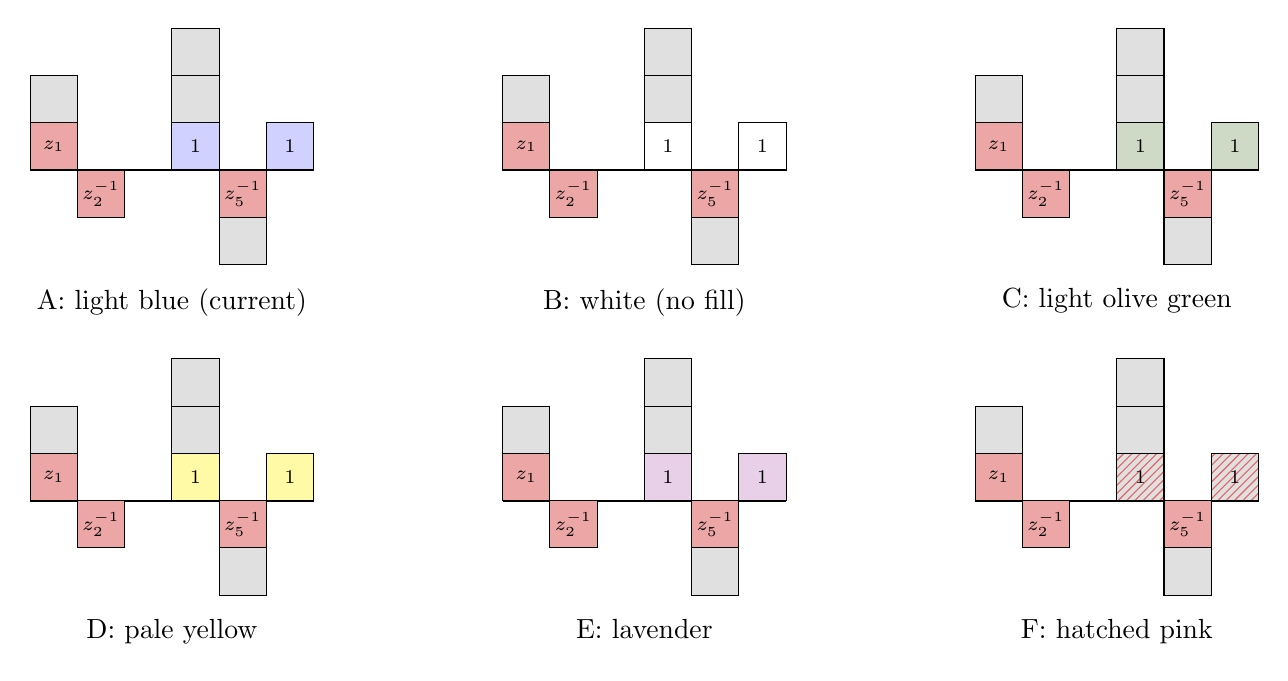
\begin{tikzpicture}[scale=0.6]
\foreach \name/\sty [count=\k from 0] in {
  {A: light blue (current)}/optA,
  {B: white (no fill)}/optB,
  {C: light olive green}/optC,
  {D: pale yellow}/optD,
  {E: lavender}/optE,
  {F: hatched pink}/optF}
{
  \pgfmathsetmacro{\X}{mod(\k,3)*10}
  \pgfmathsetmacro{\Y}{-int(\k/3)*7}
  \begin{scope}[shift={(\X,\Y)}]
  \draw[line width=0.8pt] (0,0) -- (6,0);
  \foreach \c/\h in {1/2,4/3,6/1}
    \foreach \r in {1,...,\h}
      \draw[fill=black!12] (\c-1,\r-1) rectangle (\c,\r);
  \foreach \c/\h in {2/1,5/2}
    \foreach \r in {1,...,\h}
      \draw[fill=black!12] (\c-1,-\r) rectangle (\c,-\r+1);
  \draw[fill=uibred!35] (0,0) rectangle (1,1);
  \draw[fill=uibred!35] (1,-1) rectangle (2,0);
  \draw[fill=uibred!35] (4,-1) rectangle (5,0);
  \foreach \c in {4,6} \draw[\sty] (\c-1,0) rectangle (\c,1);
  \node[font=\scriptsize] at (0.5,0.5) {$z_1$};
  \node[font=\scriptsize] at (1.5,-0.5) {$z_2^{-1}$};
  \node[font=\scriptsize] at (3.5,0.5) {$1$};
  \node[font=\scriptsize] at (4.5,-0.5) {$z_5^{-1}$};
  \node[font=\scriptsize] at (5.5,0.5) {$1$};
  \node[anchor=north] at (3,-2.3) {\name};
  \end{scope}
}
\end{tikzpicture}
\end{document}
